
\documentclass[10pt,letterpaper]{article}
\usepackage{cogsci}

\usepackage[nodoi]{apacite}
\usepackage{graphicx, subcaption}
\usepackage{amsmath}
\usepackage[american]{babel}
\usepackage[section]{placeins}

\usepackage{soul} % for \hl

\usepackage{pslatex}
% \usepackage{multirow}

\title{Desirable difficulties in the development of active inquiry skills}

\author{
  {\large \bf George Kachergis, Marjorie Rhodes, \& Todd Gureckis} \\
  \{george.kachergis, marjorie.rhodes, todd.gureckis\}@nyu.edu \\
  Department of Psychology, New York University \\
  New York, NY
}

\begin{document}

\maketitle

\begin{abstract}
This study explores the basic cognitive operations underlying the ability to ask informative questions.  We hypothesized an intrinsic link between the ability to update beliefs in light of evidence and the ability to ask informative questions. To study the developmental trajectory of this behavior, four- to ten-year-old children played an iPad game asking them to identify a hidden bug. Learners could either ask about individual bugs, or make a series of feature queries (e.g., ``Does the hidden bug have antenna?'') that could more efficiently narrow the hypothesis space. Critically the task display either assisted children with integrating evidence with the hypothesis space or required them to update it themselves.  Although we found that helping children update their beliefs improved some aspect of the active inquiry behavior, children forced to track their belief updating asked questions that were more context-sensitive and thus informative.  The results show how making a task more difficult may actually improve children's active inquiry skills, a type of desirable difficulty.

\textbf{Keywords:} 
question asking, information search, active inquiry, hypothesis testing, scientific reasoning
\end{abstract}


\section{Introduction} 


% GK: all of this stuff is well-written and somewhat relevant, but we prob don't need 6 paragraphs of general intro...help me delete? 
% I'm tempted to say: Figuring out how to efficiently navigate a hypothesis space--from learning the diagnostic features to asking the appropriate questions to appropriately updating the space in the face of new evidence--is an essential part of science, and of life, in general. So this is what we do.
A central aim of science education is to teach students how to approach the task of understanding their environment. Rather than teaching only a catalogue of facts about the biological and physical worlds, current standards emphasize teaching the conceptual and analytic skills that underlie science: detecting patterns in environments that initially appear chaotic, abstracting the general principles that can be used to understand and predict events, and importantly learning how to ask informative questions to reveal these patterns and principles when they are not immediately obvious \cite{Bransford:2000,Donovan:2005,Duschl:2007}. 

%These aims guide even the earliest, most foundational components of science education. In order to discover knowledge, whether in a real science experiment or merely when figuring out a new toy or gadget, children must learn: 1) which observable features are relevant to test, 2) how to intervene on the world in a context-sensitive manner in order to gather additional information about hidden feature values, and 3) how to integrate new evidence to update their hypothesis space.

%%Children's developing abilities to engage in these basic steps of scientific thinking are on full display in informal science learning environments, such as at science and children's museums. Indeed, a central goal of these environments is to provide children with hands-on opportunities to learn from their own explorations, to enable them to gain active experience with the steps of scientific investigation, to discover new knowledge, and to develop enthusiasm for and interest in science \cite{Bell:2009,Fenichel:2010}. As a result, we believe that informal science environments provide an excellent domain in which to explore the psychological processes related to the development of understanding.

% only keep all the sensemaking framing in the journal paper?? JOURNAL
%Informal science learning rests on the cognitive capacity for ``sensemaking'' \cite{Renner:2011}. Sensemaking, as it is understood in the cognitive and human-computer interaction literature, refers to the process of generating meaningful explanations or understandings for possibly incomplete or noisy data patterns in the environment \cite{Russell:1993,Klein:2006a,Klein:2006b}. In contrast to simple pattern recognition or categorization, sensemaking is a highly-volitional process that involves the continual evaluation of new evidence or data, and repeated information gathering. As such, the cognitive processes underlying sensemaking are often conceptualized a loop where one component process feeds into the next in a repeating sequence.
% (see Figure~\ref{fig:sensemaking_loop}).

%\begin{figure}[!h]
  %\centering
  %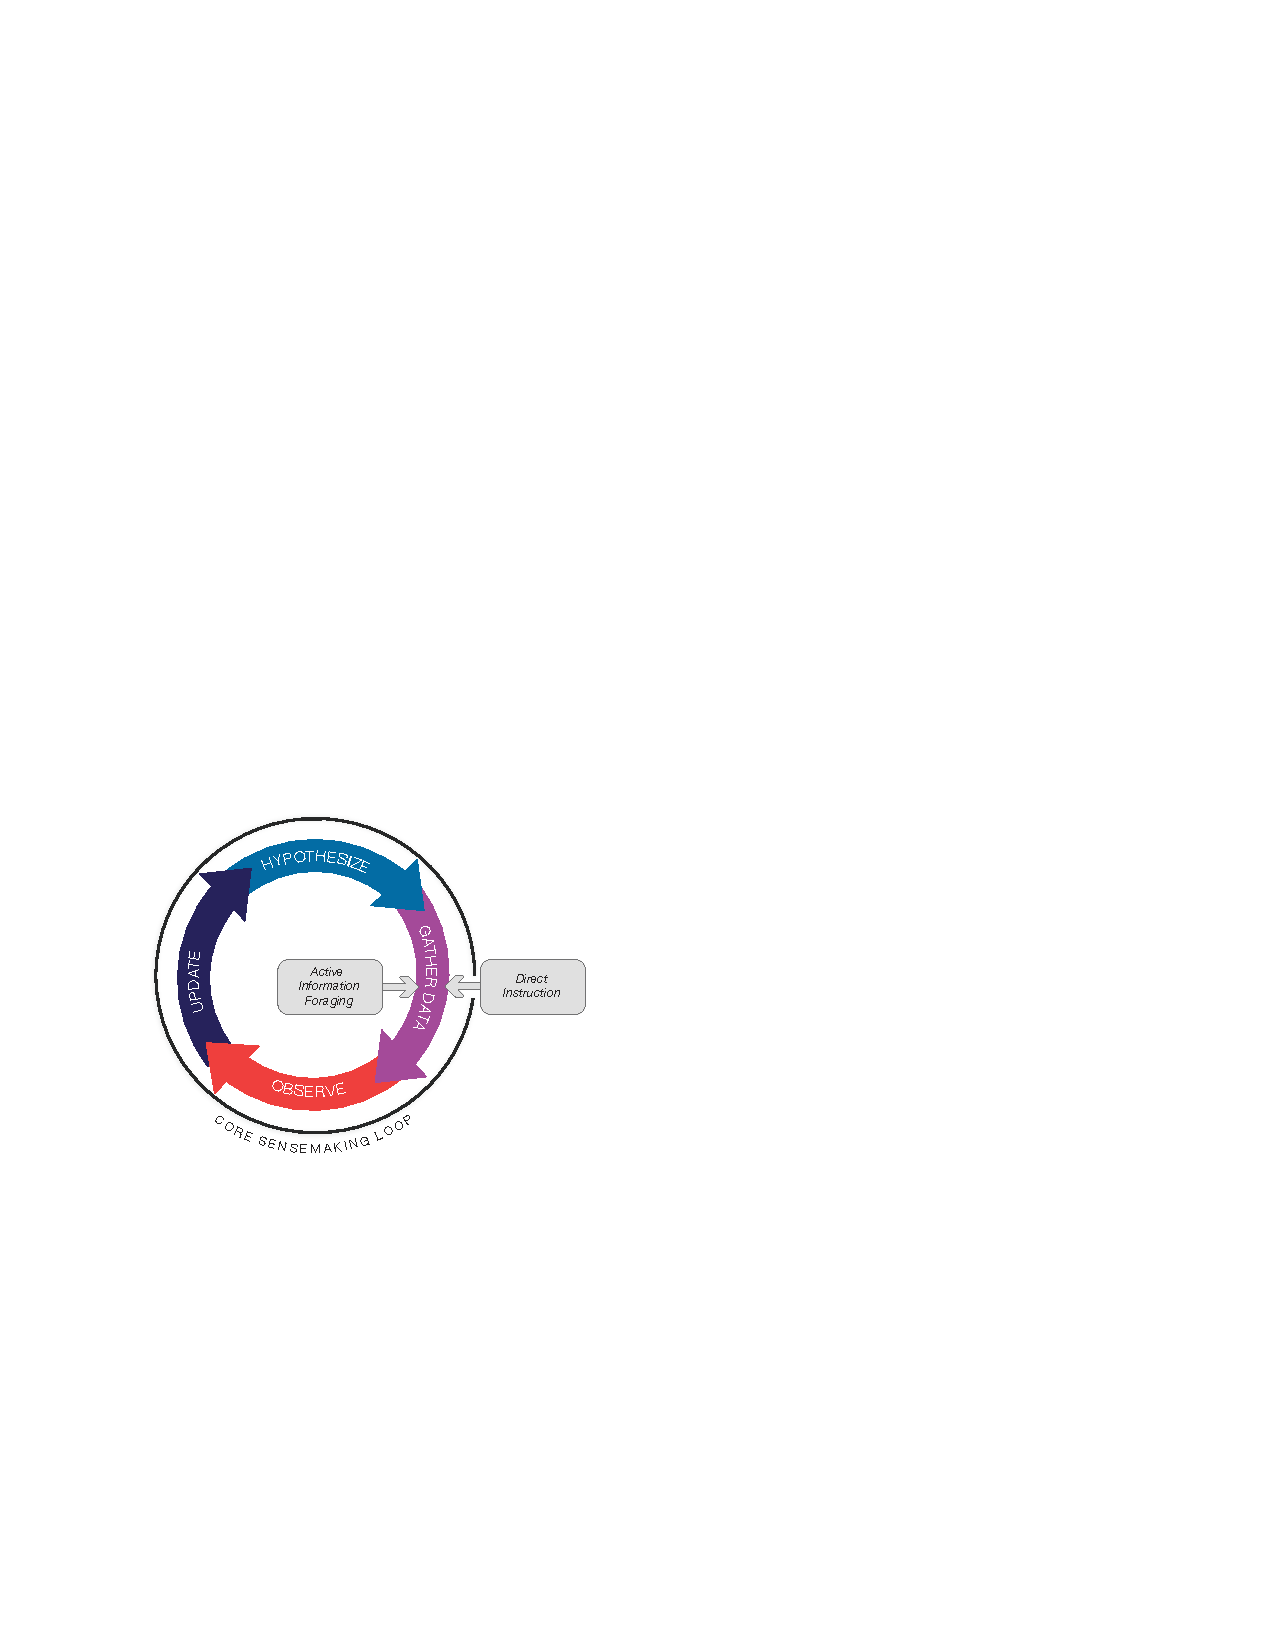
\includegraphics[width=0.45\textwidth]{figures/sensemaking_loop}
 % \caption{The sensemaking loop depicts the successive cognitive process that are engaged when attempting to derive a meaningful understanding of an initially ambiguous situation. The stages of the loop closely mirror the process of scientific reasoning engaged by scientists. However, a similar set of inductive processes are at play in many real-world situations (e.g., working an unfamiliar ATM machine, reading a complex nutrition label).}
%  \label{fig:sensemaking_loop}
%\end{figure} 

%While the sensemaking loop just described is fairly abstract, the goal of the present study is to test and elaborate this theory with the aim of better understanding how to structure formal and informal learning experiences in developmentally appropriate ways. 
% JOURNAL
%This basic sensemaking framework can be instantiated as a computational information processing model \cite{Gureckis:2012,Gureckis:2009,Markant:2012}. The advantage of this formal model is that it allows detailed, testable predictions about behavior. The model-based theory suggests possible bottlenecks that might serve as developmental limitations on learning. For example, young learners may be able to correctly update their beliefs about a set of hypotheses given a set of data, but have trouble using the remaining hypothesis space to guide future information search. This study explores the development of the data-gathering and updating stages in children, with the aim of developing a more complete understanding of the learning abilities of young children.

Many of the cognitive skills required for active scientific inquiry follow protracted developmental trajectories. For example, in tasks designed to assess scientific reasoning abilities, children in the older elementary school years (ages 8-10) often have difficulty adopting systematic strategies, such as testing the effects of one variable at a time or selecting interventions that will lead to determinate evidence \cite{Chen:1999}. Although children in the older elementary school years can be taught to engage in these strategies via direct instruction \cite{Klahr:2004,Kuhn:2005}, it is notable how difficult it is for them to discover and implement them on their own. 
%Despite the lengthy developmental trajectory of children's scientific reasoning skills, the roots of these abilities are observable even in the early preschool years. For example, in simple causal reasoning tasks, preschool-aged children can distinguish confounded from unconfounded evidence to draw causal inferences \cite{Gopnik:2001,Kushnir:2005,Kushnir:2007,Schulz:2004}. Preschool-aged children also selectively explore confounded evidence in their own exploratory play \cite{Cook:2011,Gweon:2008,Schulz:2007}. Thus, preschool-aged children show early emerging abilities to explore evidence strategically, distinguish confounded from unconfounded evidence, and to engage in causal inference from limited samples.

Active inquiry depends on the coordination of a variety of component cognitive processes.  For example, according to one popular view, learners must generate possible hypotheses to explain their environment.  They then must engage in decision making to ask questions or more effectively gather additional information.  They then must understand the results of these inquiry behaviors and update their beliefs accordingly.  The process then repeats with new hypotheses.  The various stages of this loop closely mirror the process of scientific reasoning engaged by scientists~\cite{Russell:1993,Klein:2006a,Klein:2006b}. However, a similar set of inductive processes are at play in many real-world situations (e.g., working an unfamiliar ATM machine, reading a complex nutrition label).

Bottlenecks for any of these interrelated processes my server as developmental limitations on active inquiry.  For example, young learners may be able to correctly update their beliefs about a set of hypotheses given a set of data, but have trouble using the remaining hypothesis space to guide future information search. This study explores the development of the data-gathering and updating stages in children, with the aim of developing a more complete understanding of the learning abilities of young children.


%A critical prediction of this 
%This basic sensemaking framework can be instantiated as a computational information processing model \cite{Gureckis:2012,Gureckis:2009,Markant:2012}. The advantage of this formal model is that it allows detailed, testable predictions about behavior. The model-based theory suggests possible bottlenecks that might serve as developmental limitations on learning. For example, young learners may be able to correctly update their beliefs about a set of hypotheses given a set of data, but have trouble using the remaining hypothesis space to guide future information search. This study explores the development of the data-gathering and updating stages in children, with the aim of developing a more complete understanding of the learning abilities of young children.
%
%The present study offers a fine-grained analysis of how question asking develops between the rudimentary abilities of kindergartners and the more sophisticated scientific reasoning skills of older children. This study tests children's abilities to consider plausible hypotheses, gather and evaluate useful evidence, and update their beliefs in response to new information. In this study, we test the effect of varying the degree of automation in the hypothesis updating step. By manipulating the amount of responsibility participants are given in hypothesis updating, we identify strengths and limitations of children's strategies and abilities, and characterize how they change with age. 

\subsection{The Structure of Inquiry}

The experimental framework used here is a variant of the ``20 questions'' game, in which the asker (participant) tries to ascertain what object the answerer (experimenter) is thinking of (e.g., ``What have I got in my pocket?'') by choosing and asking a minimal series of yes-or-no questions. Variants used in experiments often present a finite set of familiar kinds of objects, such as animals \cite{Ruggeri:2015front} or people \cite{Nelson:2014}, from which the to-be-discovered answer is randomly selected, and some even provide lists of acceptable questions for askers to choose from. Investigating children aged 6-11 years, \citeA{Mosher:1966} identified two broad question types used in 20 questions: \emph{hypothesis-scanning} questions test a single hypothesis (e.g., ``Handses?''), whereas \emph{constraint-seeking} questions can constrain the hypothesis space faster by querying features that are present or absent in multiple objects (e.g., ``Is it soft?''), but that do not directly identify the answer (except by elimination). \citeA{Mosher:1966} identified a developmental trajectory: 6-year-olds tend to do more hypothesis-scanning, while older children (e.g., aged 11) use more constraint-seeking questions, and also tend to find the answer after fewer questions. One explanation given for this is that only older children have developed the ability to focus on the high-level features that group the hypotheses, whereas younger children focus on individual stimuli \cite{Mosher:1966,Ruggeri:2015front}. However, \citeA{Herwig:1982} found that when items were drawn from basic-level categories (e.g., airplane, bed, lamp), even 6-year-olds increased their rate of asking constraint-seeking questions if first asked to sort the items that go together. In the same vein, \citeA{Ruggeri:2015front} also found that appropriate cueing can increase the use of constraint-seeking questions: this effect was seen after objects were described using basic-level terms instead of exemplar names. (animals)

\citeA{Nelson:2014} studied a 20 questions task using another familiar domain: people that varied on familiar features (e.g., gender, hair color, etc.). That study showed 8-10 year-old children searched adaptively, in the sense that they tended to ask questions about features that appear often in the real world, and that roughly bisect the search space. Our study asks if and when children are able to learn these feature distributions in an unfamiliar hypothesis space, and whether they are able to use this knowledge to efficiently search that space.

However, these studies all used hypothesis spaces that were likely familiar to participants to some extent---and likely to a larger extent for older participants. 
In contrast, the present study introduces a novel, hierarchically-structured hypothesis space in which the concrete features are randomly assigned. 


How do kids choose queries to search a hypothesis space? We study belief updating and information seeking as a function of age, along with how strategies for acquiring information change within individuals.

 %\citeA{Ruggeri:2014} found that younger and older children ask more constraint-seeking questions when the hypothesis space is large--as they normatively should. 
 \citeA{Ruggeri:2015} studied 7-8 year-olds, 9-11 year-olds, and 17-18 year-olds asking questions to identify the cause of an event in real-world scenarios (e.g., Why is a man late to work?). All age groups in that study used more constraint-seeking questions when hypothesis-scanning was unwise: e.g., when the problem had a large hypothesis space or when not all solutions were equiprobable. The present study differs from that of \citeA{Ruggeri:2015} in several ways, among them being that the present task: 1) is not a causal inference task, 2) introduces a novel hypothesis space with features' informativeness being randomly assigned, and 3) presents the available strategies (i.e., hypothesis-scanning and constraint-seeking queries) explicitly as side-by-side buttons.

In this study, children (ages 5-10) play multiple rounds of a self-guided 20-questions style iPad game with a structured but novel hypothesis space. We assess how well they monitor their own understanding and how they choose to seek additional information until their understanding is complete. Specifically, we ask how children test hypotheses when they can use a mixture of hypothesis-scanning and constraint-seeking questions in a novel feature space: Do they use feature queries and then scan hypotheses? Do they gradually learn to test more discriminative features? Do they make queries that are context-sensitive (i.e., relevant to the information state they are currently in)? Does manually updating the hypothesis space reveal bottlenecks, or perhaps push learners to find more informative queries?


\section{Experiment}

The purpose of the experiment is to investigate how children utilize hypothesis-scanning and constraint-seeking questions when trying to discover a hidden feature in a novel environment, and to ask whether evidence-based belief-updating is a bottleneck in the knowledge discovery process. To address these issues, we created a tablet-based game in the ``20-questions'' style (or more specifically, ``Guess Who?''). Formally, this task involves search of a binary decision tree. To accomplish this search optimally, one should search for and query the feature at each step that most nearly bisects the hypothesis space.

\subsection{Methods}

\subsubsection{Participants}

Participants in this experiment were 132 children between the ages of 5 and 10 years old who were recruited at the American Museum of Natural History's Discovery Room.

\subsubsection{Stimuli}

On each round, 16 beetles (i.e., bugs) with the same body shape were used as stimuli. Bugs were defined by the presence or absence of 9 features: green body, orange eyes, antennae, big spots, tiny spots, legs, leaves, water droplets, and blue ``fur''. Two examples are shown in Figure~\ref{fig:example_bugs}. Each of these features was represented on a button, available for participants to query. Before participants were allowed to begin, the experimenter explained at least three of these buttons, randomly selected. An additional feature button depicted a particular body shape that was not relevant to the bugs on display. The hidden bug was randomly selected on each round, and each round had differently-shaped bug bodies, selected from a pool of 16 unique body shapes.

\begin{figure}[h]
  \centering
  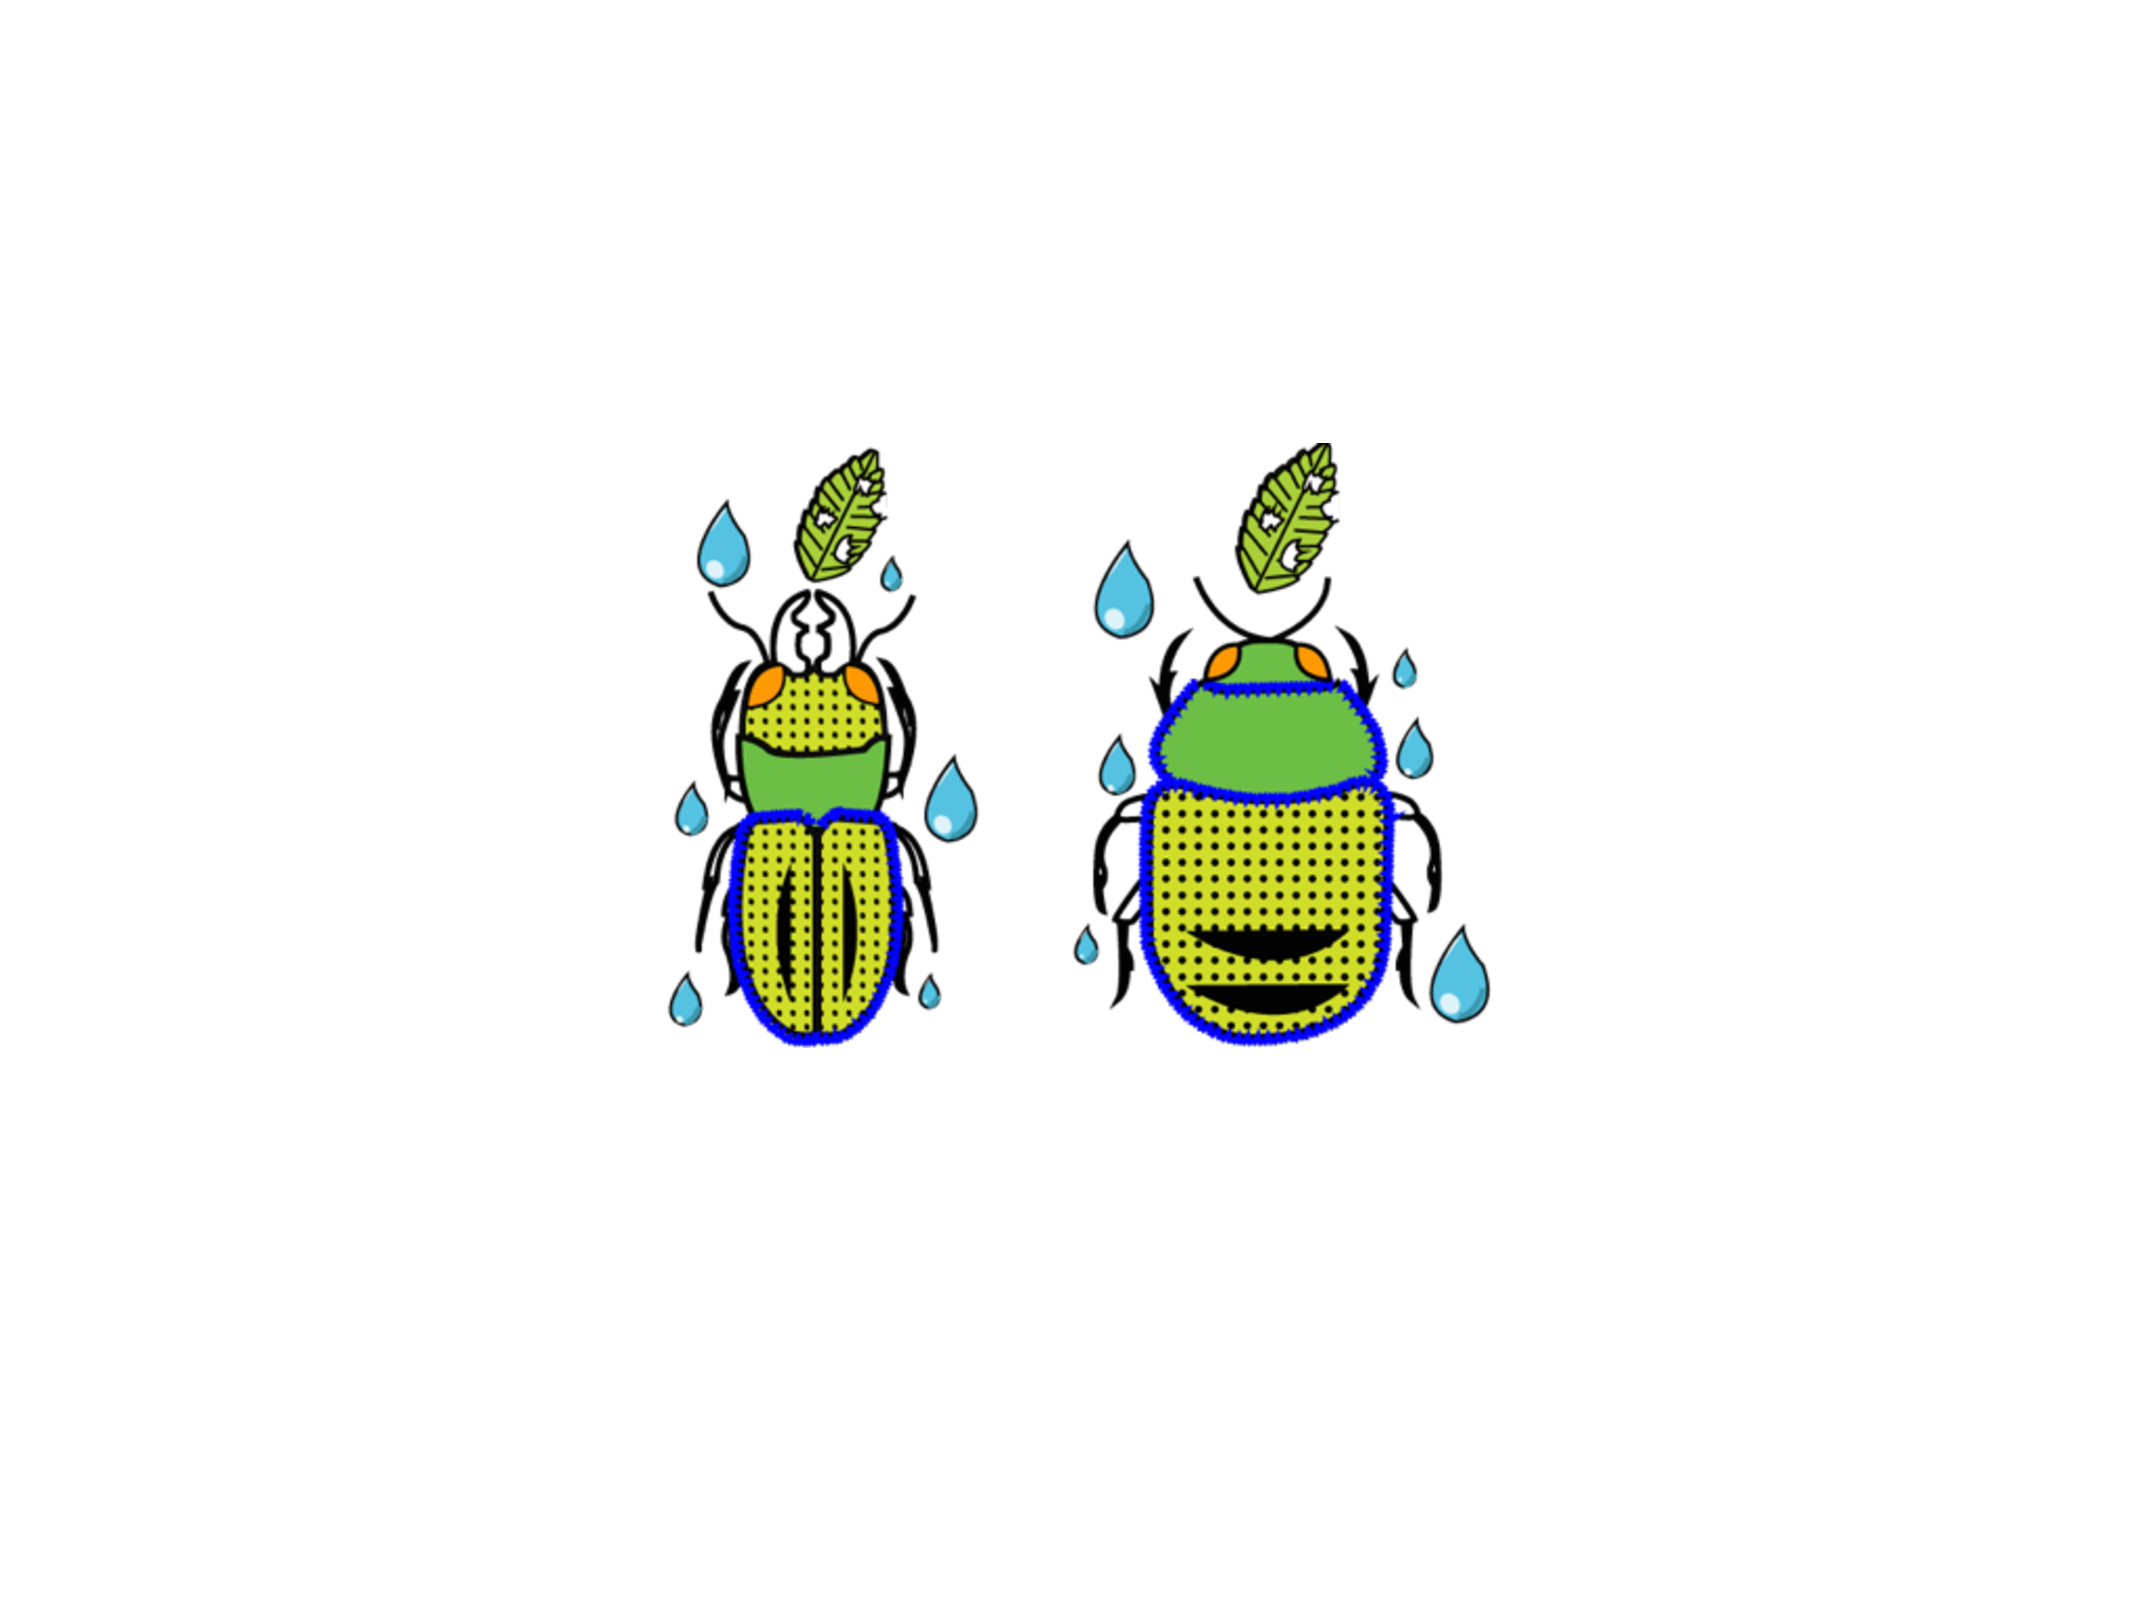
\includegraphics[width=0.22\textwidth]{figures/example_bugs}
  \caption{Example bug types with all nine of the binary features present. One of 16 bug body shapes was used per round.}
  \label{fig:example_bugs}
\end{figure} 

The features were not uniformly distributed: some were more frequent than others (relevant to a maximum of eight bugs), while some were very infrequent (relevant to a minimum of 1 bug), with the partially-nested structure shown in Figure~\ref{fig:feature_table}. Thus, an efficient participant will choose a feature that is found on half of the bugs remaining onscreen. The abstract features in Figure~\ref{fig:feature_table} were randomly assigned to the visual features for each participant, and then remained consistent across rounds. This gave participants the opportunity to learn the structure across rounds, for example to perhaps figure out which visual features are most relevant to ask about first.

\begin{figure}[h]
  \centering
  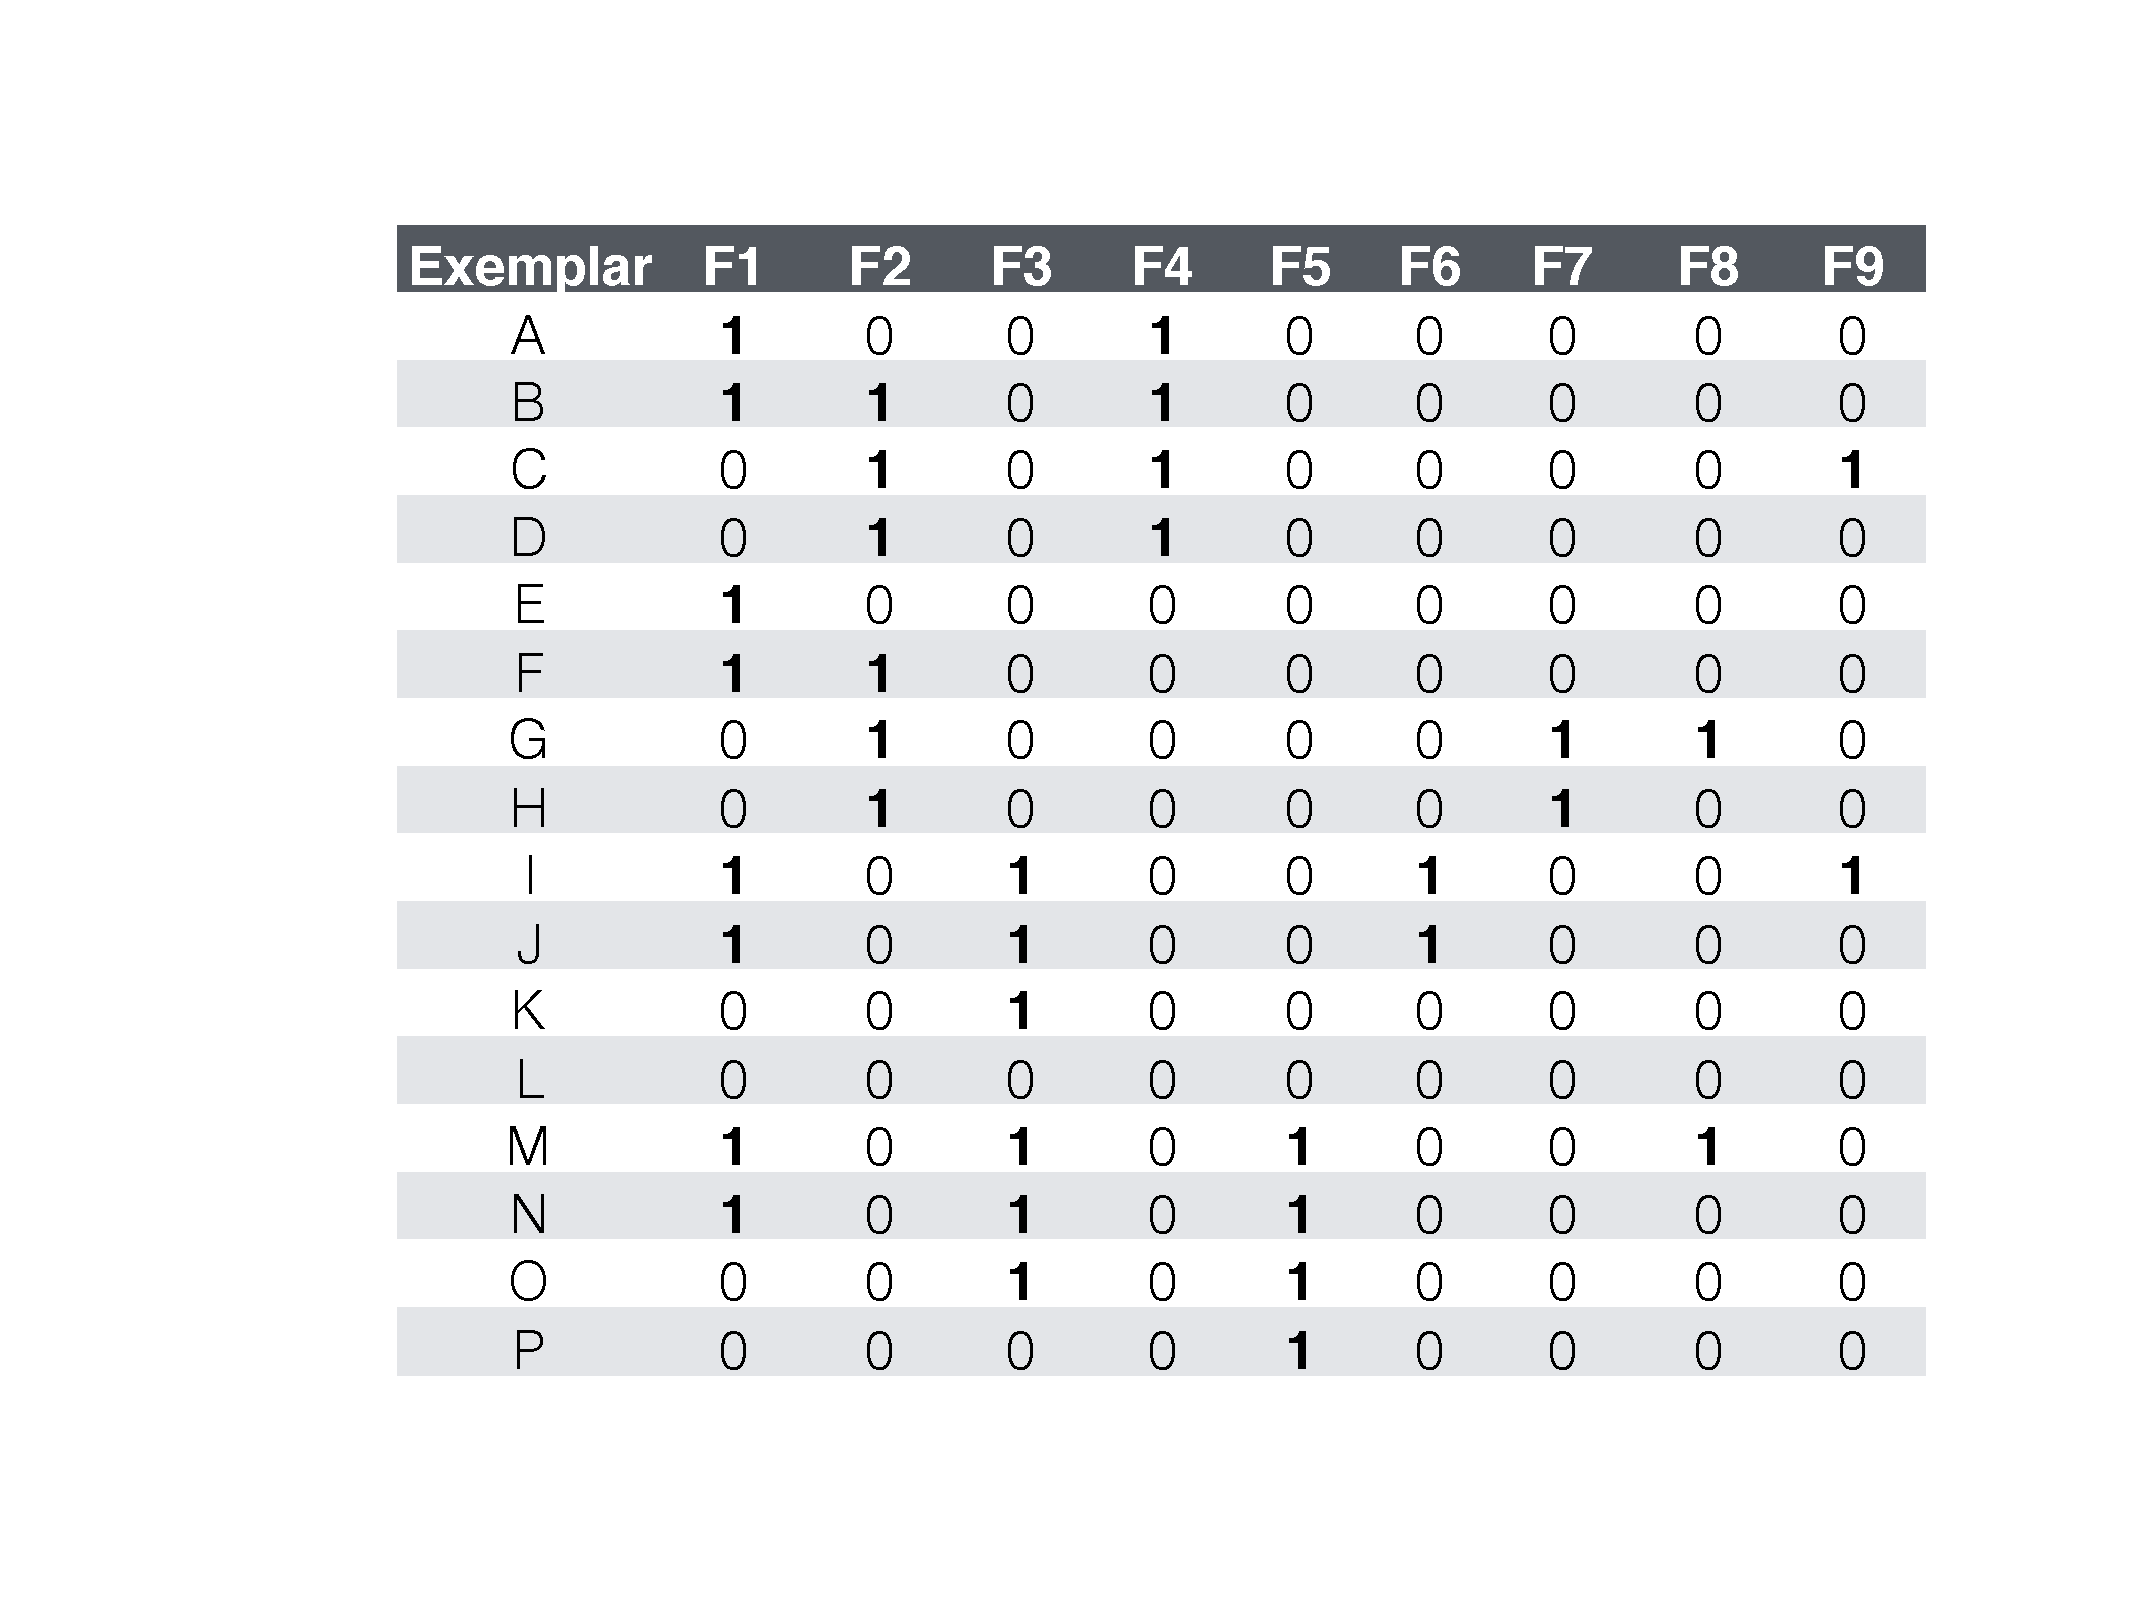
\includegraphics[width=0.48\textwidth]{figures/feature_table}
  \caption{The abstract feature structure of the 16 exemplars used in each round. Each participant had these abstract features randomly assigned to the visual features, but had a consistent assignment used round-to-round.}
  \label{fig:feature_table}
\end{figure} 

\subsubsection{Procedure}

After being trained by an experimenter on a simpler version of the task with unrelated stimuli (a dog trying to find it's house), participants played 5 or more rounds of an iPad game asking them to identify which one of 16 bugs is hidden under a rug (see Figure~\ref{fig:task-overview}). The task alternates between the query phase and the elimination phase. In the query phase, players can either query individual bugs, or use feature queries (e.g., ``Is the hidden bug green?'') to find out whether the hidden bug has a particular feature. If a single exemplar is queried by tapping on it, feedback is immediate: if it happens to be the hidden bug, a smiley face appears and the round is done, whereas if the tapped exemplar is not the hidden bug, a red ``X'' is shown on top of the tapped bug and the bug becomes grayed out (i.e., eliminated). After a feature query, the bug gives feedback, saying ``Yes!'' (it has the feature; narrated by the experimenter), or ``No!'' (it does not have the feature). It is now the elimination phase, during which bugs that are inconsistent with the feedback are eliminated, and the hypothesis space is thus narrowed. Participants were assigned in counterbalanced order to one of two hypothesis-updating conditions. In the automatic-update condition, after the feedback from a feature query, subjects merely press the ``Eliminate'' button and the irrelevant bugs are eliminated (grayed out), and the game returns to the guessing phase. In the manual-update condition, after a subject makes a feature query and sees feedback, they must select each bug that is consistent with the feedback for that feature, as shown in the top right of Figure~\ref{fig:task-overview}. Bugs are selected by tapping, and can be deselected by tapping again. Only when participants were done selecting bugs did the experimenter press the ``Eliminate'' button, which eliminated any bugs that were not selected. Although manual-update participants received training for the manual elimination in the dog house training task, as well as gentle reminders in the first round of the bug game, it should be noted that it is possible for mistakes to be made during manual updating--unlike in the automatic condition.

\begin{figure}[h]
  \centering
  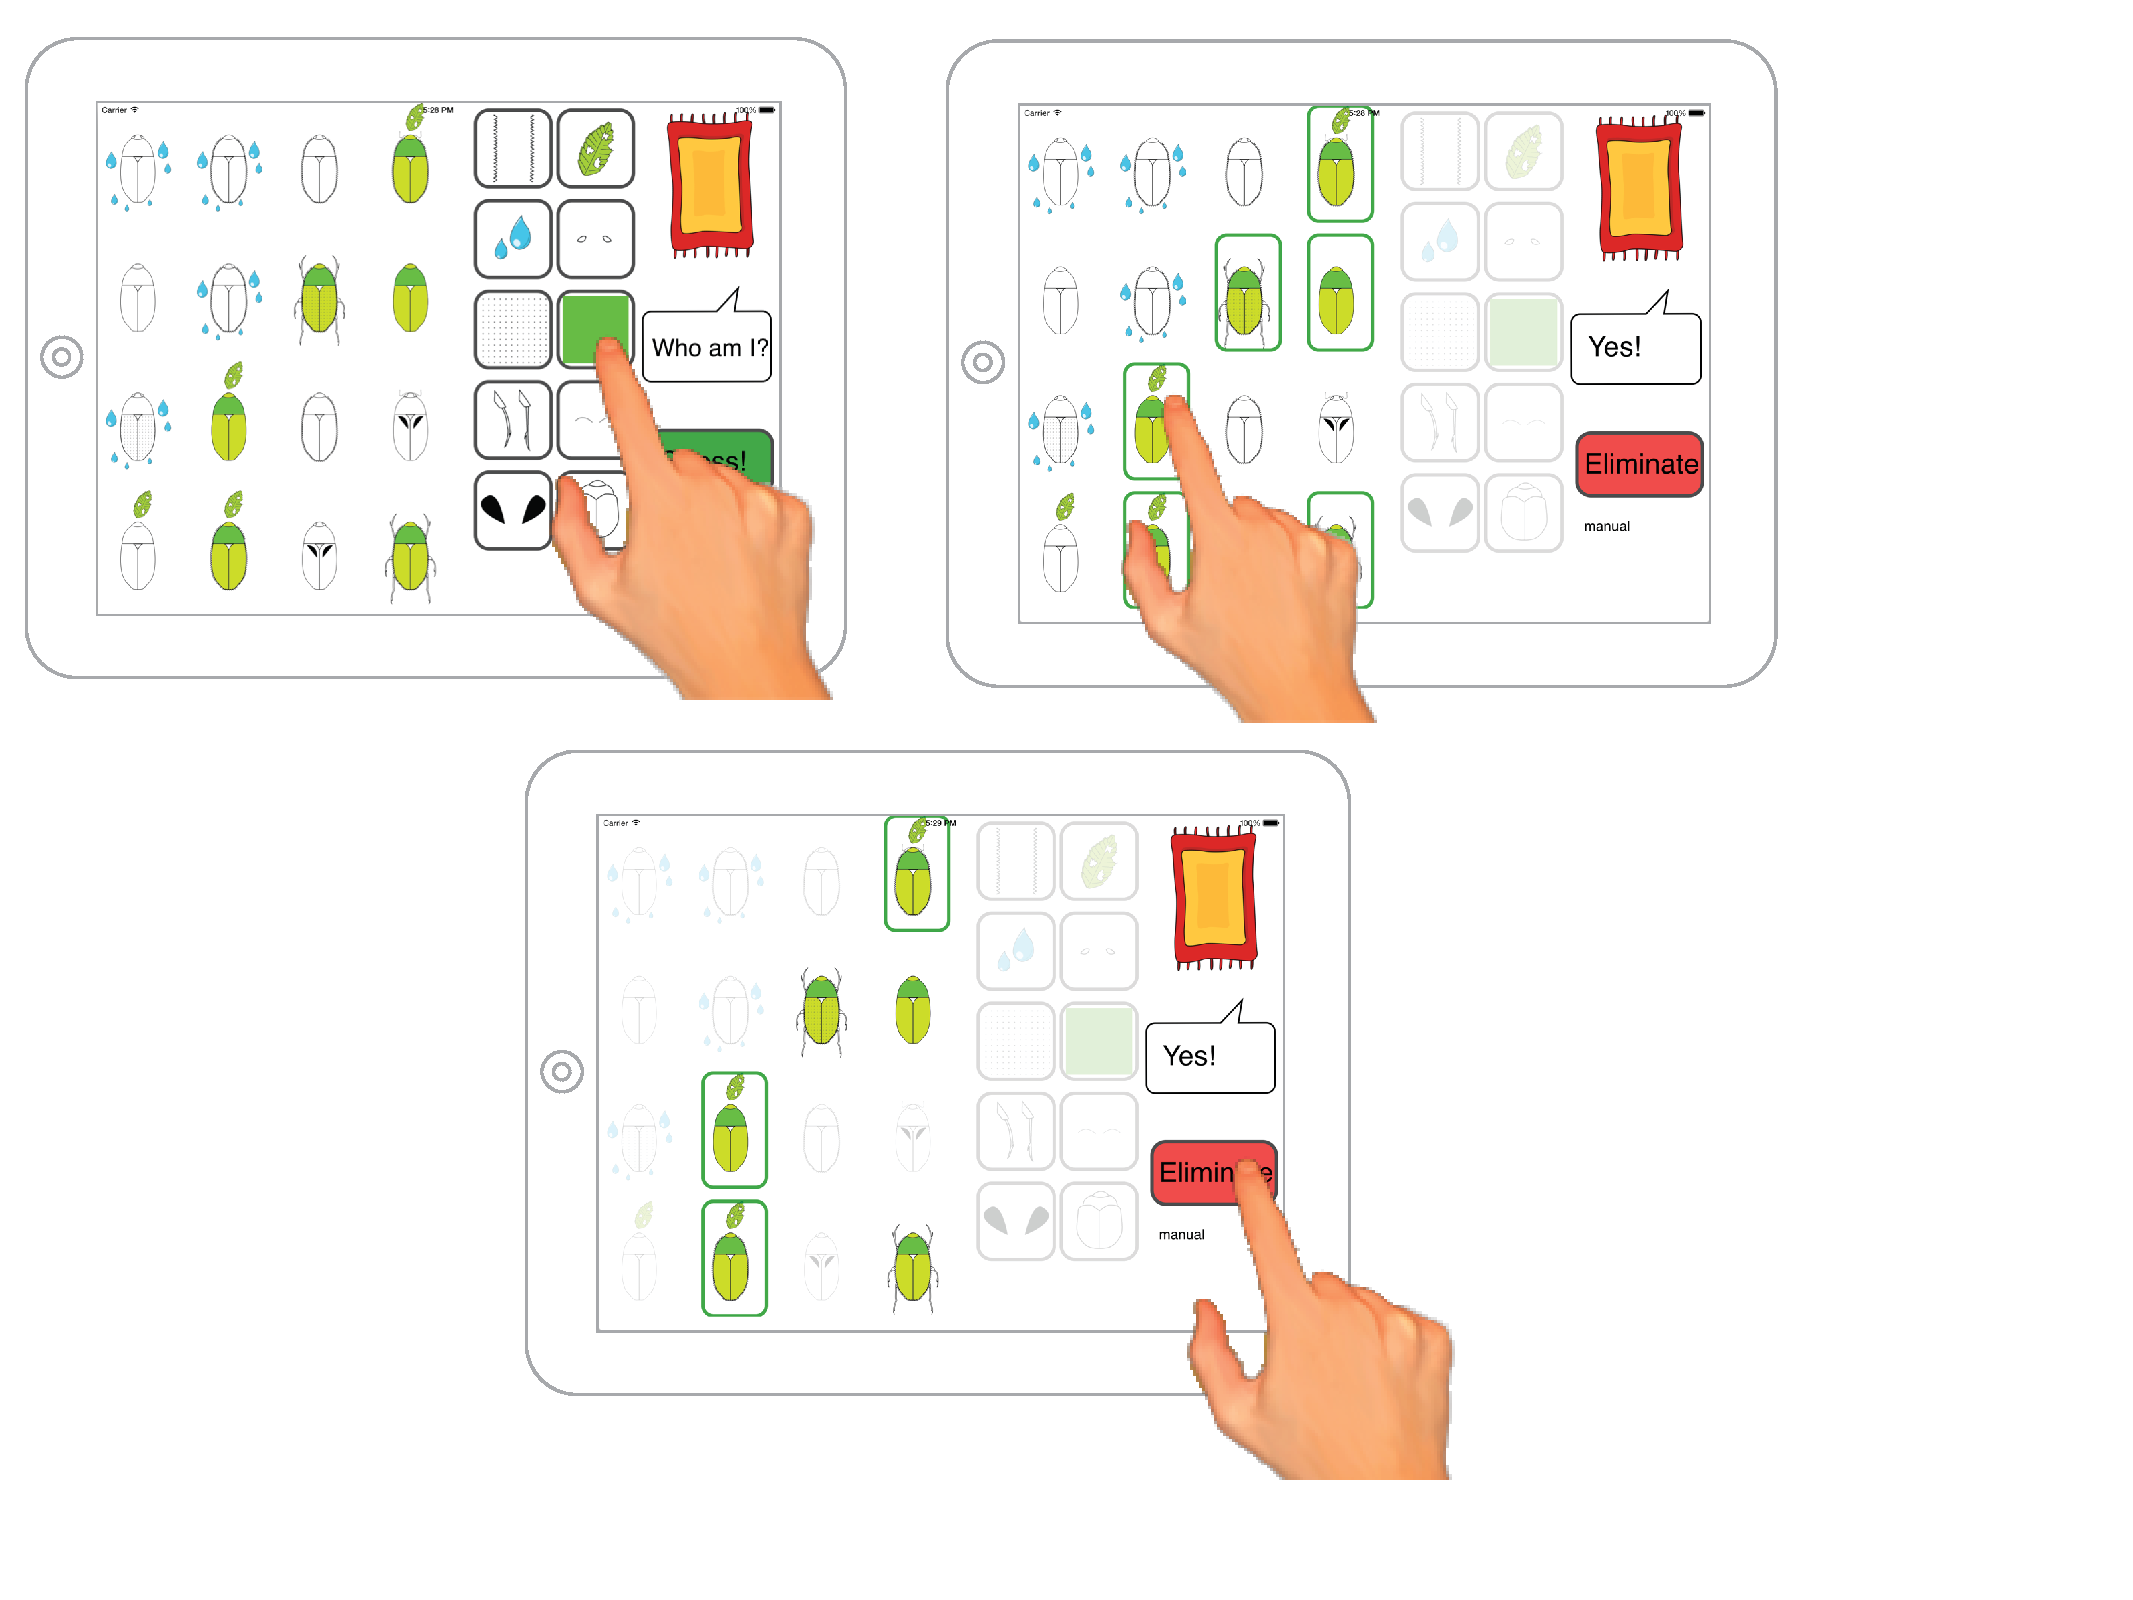
\includegraphics[width=0.5\textwidth]{figures/task_overview}
  \caption{Task overview: in the upper left, a feature button is used, asking if the bug hidden under the rug is green. Given feedback (``Yes!''), participants in the manual update condition select the bugs that are consistent with this new information (upper right), whereas in the automatic condition the consistent bugs are selected by the game. Players in both conditions press the red button to return to the button phase, and again either choose a feature button or query a single bug.}
  \label{fig:task-overview}
\end{figure} 


\subsection{Results}

\subsubsection{Overall}

Of the 134 children recruited, we analyze the rounds from 121 children (21 5-year-olds, 20 6-year-olds, 22 7-year-olds, 20 8-year-olds, 20 9-year-olds, and 18 10-year-olds) who completed 5 or more rounds of the game. Of these 804 rounds, we analyze only the first 10 rounds (only 8 children played more than 10 rounds, but one played 51 rounds: we do not want to bias our statistics too heavily towards these outliers). Thus, we analyze 722 rounds from 121 children. On average, a round lasted 64 s (median: 45 s; sd: 56 s). The mean number of queries (feature and exemplar) taken to complete a round was 6.5 in the automatic-update condition, and 7.6 in the manual-update condition. However, the median queries taken per condition was 6: are these two distributions different? A Kolmogorov-Smirnov test of these two non-normal distributions showed that they are significantly different ($D = 0.13$, $p<.01$). Note that an optimal player requires fewer queries: an expected mean of 4.5 queries can be achieved by choosing the feature query to bisect the hypothesis space for the first three queries, and then guessing one of the two remaining exemplars (and when unlucky, finally choose the last). For comparison, we simulated 700 rounds of the game in which queries--feature and exemplar pooled--are chosen uniformly at random, without replacement. These simulated random rounds took a mean of 8.9 queries (median: 9) to complete--more than children in either updating condition. We continue to use these simulated random-choice rounds throughout the paper in comparisons to the participants' behavior.

\subsubsection{Querying Behavior}

Before we delve into the information-theoretic analysis that will ultimately reveal how efficiently participants make queries to reduce the hypothesis space, it is useful to get a better sense of the type and range of behaviors observed. What mixture of feature and exemplar queries do participants use, within and across rounds? Participants' mean number of queries per round were computed and subjected to an ANCOVA with condition and query type as factors and age and round number as covariates. This ANCOVA indicated significant main effects of condition (F(1,1312) = 14.90, $p<.001$) and age (F(1,1312) = 29.48, $p<.001$), as well as marginal main effects of round (F(1,1312) = 3.09, $p<.08$) and query type (F(1,1312) = 3.47, $p=.06$). Overall, older children require fewer total queries to complete a round, evidenced by a significant negative correlation with age ($t(119) = 2.50$, $p=.01$). Participants' mean number of feature queries made per round was 3.6, and their mean number of exemplar queries was 4.1, lower than the simulated random rounds' mean number of feature queries (6.5) and exemplar queries (5.3), but above the optimal.\footnote{Note that although there are at first more exemplars (16) than feature buttons (10) to query, after the first click or two there will likely be few exemplars remaining to click, which is why the expected number of exemplar queries is lower than the expected number of feature queries in the simulation.} 

There were significant interactions of condition and query type (F(1,1312) = 41.56, $p<.001$), age and query type (F(1,1312) = 14.45, $p<.001$), and round and query type (F(1,1312) = 11.89, $p<.001$), as well as a significant three-way interaction of condition, age, and query type (F(1,1312) = 13.39, $p<.001$). Figure~\ref{fig:clicks-per-agecond} shows the average number of query types used per round for participants of each age. Across all ages in the manual-update condition there were more exemplar queries than feature queries. In comparison to the manual condition, there were fewer exemplar queries in the automatic condition ($M_{man} = 5.0$, $M_{auto} = 3.2$, $t(103.5)=4.1$, $p<.001$), while there were more feature queries in the automatic condition ($M_{auto} = 3.8$) ($M_{man} = 3.3$, $t(102.9)=2.1$, $p<.05$). 

\begin{figure}[h]
  \centering
  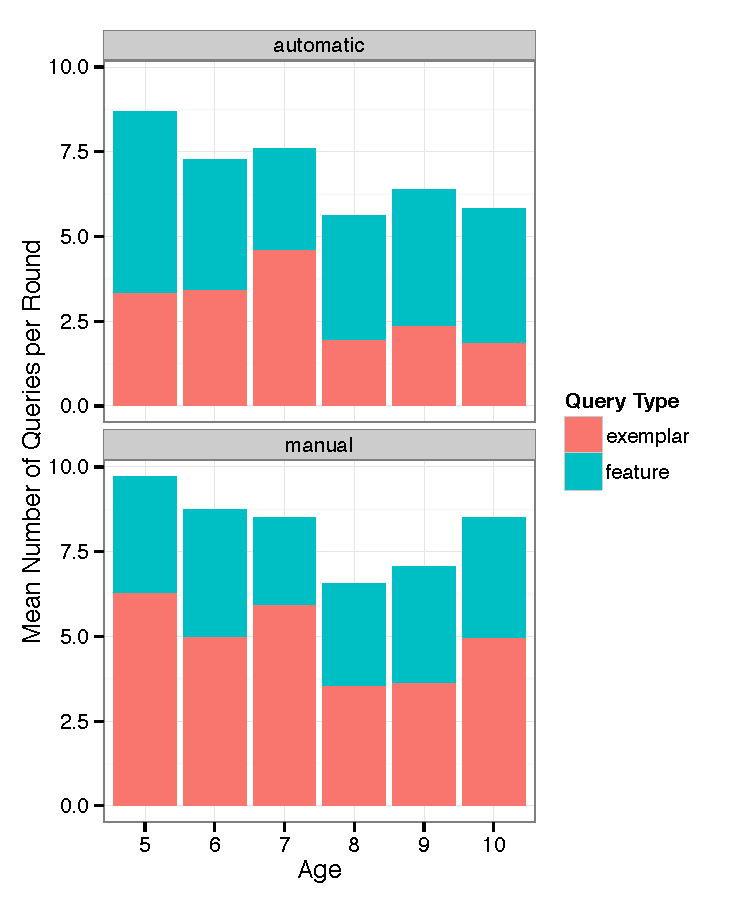
\includegraphics[width=0.49\textwidth]{figures/clicks_by_age_condition_query_type}
  \caption{Mean number of queries of each type per round by age and condition. Error bars show +/-1SE.}
  \label{fig:clicks-per-agecond}
\end{figure} 

In summary, it is clear that the manual-update condition results in fewer feature queries (i.e., constraint-seeking questions), and more reliance on exemplar queries. 
%\hl{ANCOVA on total queries per round shows advantage for age, only a marginally significant effect of round (p=.07); include or not?} 
It is reasonable to suggest that manual-update participants may be discouraged from using feature queries by at least two factors: 1) it demands more time and cognitive effort to manually update the hypothesis space after a feature query than in the automatic-update condition, and 2) the manual update process is error-prone, and any mistakes may in turn lead to more exemplar queries in order to recover. In the following analyses, we thus investigate errors in manual updating, as well as response time patterns and information theoretic analyses that will indicate whether the quality of feature queries varied in the two update conditions.

% Automatic subjects take fewer queries (6.7) than manual subjects (8.1; $t(41)=2.6$, $p=.01$). Feature query usage tends to drop off across rounds.

% \begin{figure}[!h]
% \centering
%  \includegraphics[width=0.5\textwidth]{figures/query_type_prop_by_round}
%  \caption{Proportion of feature vs. item queries by round.}
%  \label{fig:query-prop-round}
% \end{figure} 
  \vspace{.05cm}
\subsubsection{Response Times}

Participants' median RT for each button type (feature and exemplar) was computed for each round and these data were subjected to an ANCOVA with condition as a between-subjects factor, and both age and round number as covariates. This ANCOVA indicated significant main effects of button type (F(1,1317) = 5.30, $p<.05$) and age (F(1,1317) = 12.01, $p<.001$), as well as a marginal effect of condition (F(1,1317) = 3.56, $p = .06$). Overall, participants took much longer to make feature queries (7,470 ms) than to press an exemplar button (2,680 ms), perhaps indicating reluctance or greater consideration of their options for the mentally-taxing option of choosing a feature to query. There were also significant interaction effects of button type and condition (F(1,1317) = 69.62, $p<.001$); age and round number (F(1,1317) = 14.74, $p<.001$); and button type, age, and round number (F(1,1317) = 19.24, $p<.001$). Figure~\ref{fig:basic-rt} shows the mean of subjects' median RTs for each button type, split by condition. Feature queries were slower in the manual-update condition, which could indicate 1) more careful thought given to features in this condition, and/or 2) general hesitance to use feature queries, perhaps because it is time-consuming (even difficult) to manually update hypotheses. Thus, we next examine whether many errors are made under manual updating.

\begin{figure}[h]
  \centering
  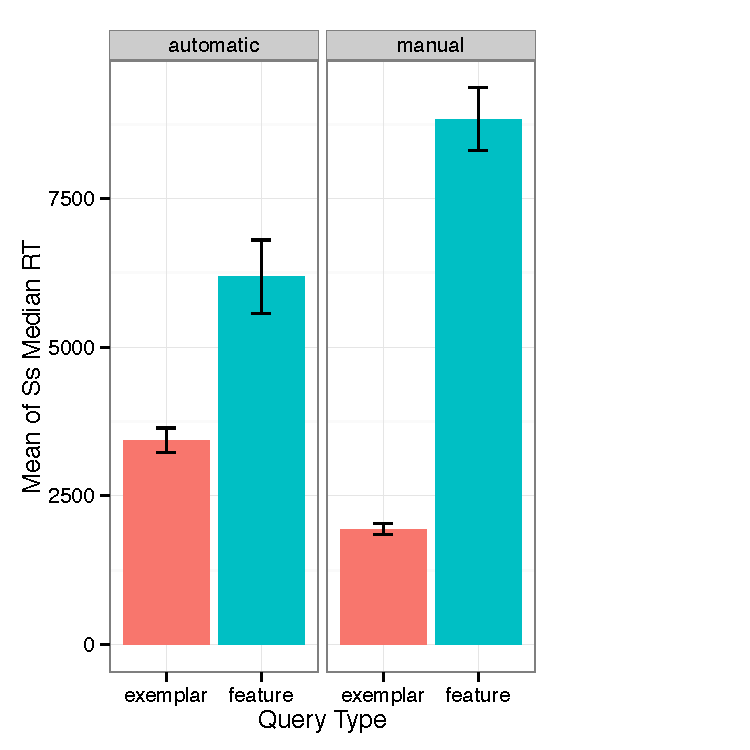
\includegraphics[width=0.33\textwidth]{figures/RT_by_condition_query_type}
  \caption{Mean of participants' median RT for each condition and query type. Exemplar queries were faster than feature queries, which represent a more complex strategy and thus likely required more thought. Feature queries were slower in the manual-update condition: it seems the difficulty of updating in this condition made participants think even more carefully about using feature queries. Error bars show +/-1SE.}
  \label{fig:basic-rt}
\end{figure} 
%\hl{maybe leave out section from conference paper...or just leave out graph?}

\subsubsection{Manual Update Mistakes}

The manual-update condition allows participants to commit two types of error during hypothesis updating: a miss is defined as a failure to eliminate a bug, and a false alarm is a failure to keep a hypothesis that was consistent with the query. Note that a miss is an error of commission--i.e., the bug had to be tapped to be kept--whereas a false alarm is an error of omission (i.e., failing to tap a bug), and thus we expect more of the latter. Comparing the manual-update subjects' mean number of errors of each type per round, indeed there were more false alarms ($M=6.9$, sd = 1.9) than misses ($M=1.8$, sd = 1.3; paired $t(58) = 19.8$, $p<.001$). A MANCOVA to determine if error rates were related to age did not find a significant effect for either misses (F(1,56) = 0.77, $p>.05$) or false alarms (F(1,56) = 0.23, $p>.05$). Given the fairly high rate of errors in manual updating, it is perhaps unsurprising that fewer feature queries and more exemplar queries were made in this condition than under automatic updating of the hypothesis space. However, RT analyses indicated that feature queries took longer under manual updating: is this just reluctance, or could it be that feature queries were more carefully considered in this condition than under the ease of automatic updating? 
% also tried with round (max of 13...but only 1 of those) and had no effect...should we only be analyzing first 5 or 6 rounds in ANOVAs??

\subsubsection{Expected Information Gain}

Each successive query reduces the size of the remaining hypothesis space to some degree. The appropriate way to analyze the contextual sensitivity (i.e., are they choosing a feature that is relevant to many of the remaining exemplars, thus quickly reducing the hypothesis space?) of participants' queries is to calculate the Expected Information Gain (EIG) of the query they made. We first introduce key terms used to define EIG. Entropy measures uncertainty about the outcome of a random variable $X$. Entropy is 0 when there is only one possible outcome, and maximal when all possible outcomes are equiprobable (i.e., a uniform distribution).

\begin{equation}
  H(X) = -\sum_{x} p(x) \cdot log(p(x))
\end{equation}

Mutual information gain measures the change in entropy as we receive a new piece of information $Y$, i.e., how much does our uncertainty about X change given that we know Y?

\begin{equation}
  I(X;Y) = H(X) - H(X|Y)
\end{equation}

The Expected Information Gain (EIG) of a query $Q$ is the weighted average of the information possible from each possible answer to the query, weighted by the current probability of receiving that answer. This will be 0 (or near-0) for queries that can be expected to eliminate none or just one or two hypotheses in a large space, and more positive for queries that are likely to eliminate a larger number of hypotheses. In this task, EIG is maximal (1) for a feature query that will eliminate half the remaining hypotheses. Such a query is always available at the beginning of any round, and due to the partially-nested feature structure used, maximal EIG queries are often available at other stages of the round.

\begin{equation}
  EIG(Q) = -\sum_{Y} p(Y|Q) I(X;Y)
\end{equation}

The EIG for each participants' feature queries\footnote{Exemplar query EIGs are less interesting, as they are a simple function of how many remaining hypotheses there are. Participants' choice of feature query, on the other hand, indicates how sensitive they are to the relevance of each feature--and to the context of their current situation.} were computed, and their mean EIG for each round were subjected to an ANCOVA with condition as a between-subjects factor, and both age and round number as covariates. This ANCOVA indicated significant main effects of condition (F(1,519) = 42.92, $p<.001$), age (F(1,519) = 4.15, $p<.05$), and round (F(1,519) = 6.33, $p = .01$), with no significant interaction effects. Figure~\ref{fig:EIG_by_age} shows mean EIG per feature query by age and condition. Mean EIG of feature queries for each subject was marginally significantly correlated with age ($t(116)=1.77$, $p=.08$, $r=.16$), showing that older children tended to use more relevant feature queries. The feature queries made by participants in the automatic condition had significantly lower EIG than those made in the manual condition ($M_{auto} = .60$, $M_{man} = .74$, $t(116) = 5.49$,  $p<.001$). Thus, although manual-update participants used fewer feature queries overall, and tended to make mistakes during hypothesis updating, the greater amount of time they spent when choosing a feature query tended to pay off: manual-update participants queried features with higher expected information gain than automatic-update participants. 
%\hl{full paper: explore click-by-click EIG in a round: is it that automatic participants don't know which feature to click even on the first click, or just that manual subjects ask more contextually-sensitive questions, choosing more informative features after the first click? (it's the latter)}

%\begin{figure}[!h]
%  \centering
%  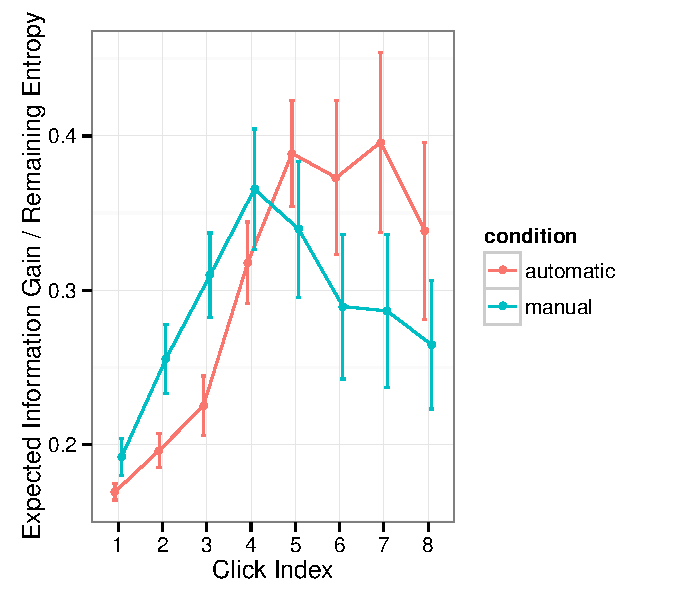
\includegraphics[width=0.49\textwidth]{figures/info_gain_prop_by_click}
%  \caption{Mean expected information gain (of feature queries only?) by click index, for all rounds, per condition. Bars show +/-1SE.}
%  \label{fig:EIG_by_click}
% \end{figure} 

%\begin{figure}[!h]
%  \centering
%  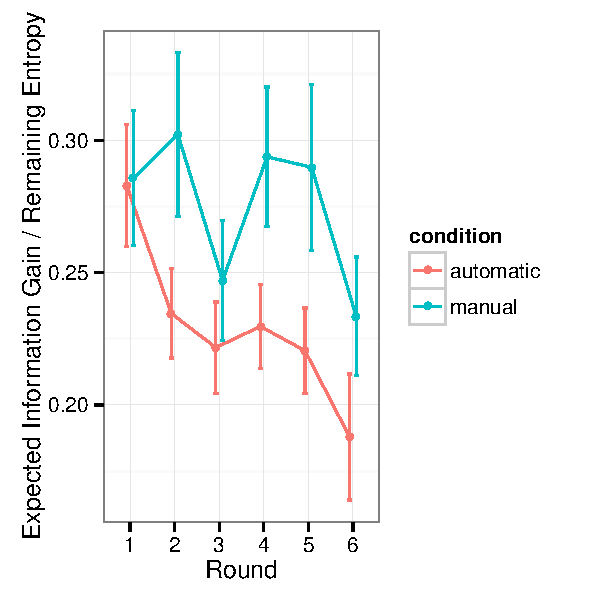
\includegraphics[width=0.49\textwidth]{figures/info_gain_prop_by_round}
%  \caption{Mean expected information gain (of feature clicks only?) by round for each condition. Bars show +/-1SE.}
%  \label{fig:EIG_by_round}
%\end{figure} 

\begin{figure}[t]
  \centering
  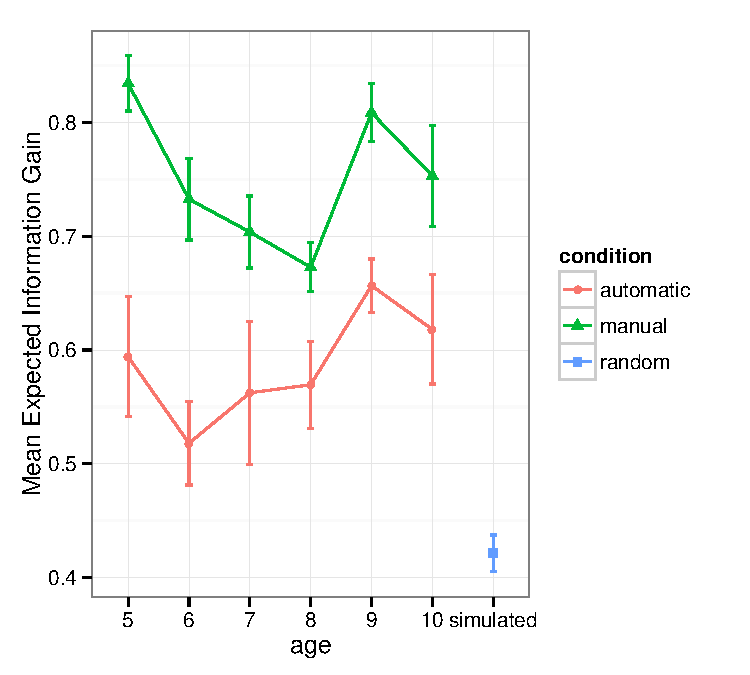
\includegraphics[width=0.49\textwidth]{figures/EIG_by_age_n_condition}
  \caption{Mean expected information gain for feature queries by age and condition, with simulated subjects making random feature queries for comparison. Manual-update subjects had higher EIG than automatic-update subjects, and both were better than random--but suboptimal (~1). Bars show +/-1SE.}
  \label{fig:EIG_by_age}
\end{figure} 

\subsubsection{Individual Variation and By-click Analyses}

%Do participants start a round by making a feature query? After how many feature queries--or when how many hypotheses remain--do they switch to making exemplar queries?

%\hl{maybe only in full paper?}
%Individual strategies: mostly exemplar vs. feature queries? Do they use consistent feature buttons across rounds?

In both conditions, the first three clicks are more likely to be feature than exemplar queries (see Figure~\ref{fig:query-prop-click}), and automatic-update subjects often make a fourth feature query before likely moving to exemplar queries. Both human conditions are quite different than the simulated random subjects, looking more like the optimal sequence: 3 feature queries and then one (sometimes two) exemplar queries. 
%Feature queries are made at a rate that is correlated with the number of exemplars they are relevant to ($r=.79$, $t(8)=3.6$, $p<.01$). 
% \hl{...maybe simulate based on the human choice probabilities, and compare EIG?}

\begin{figure}[h]
  \centering
  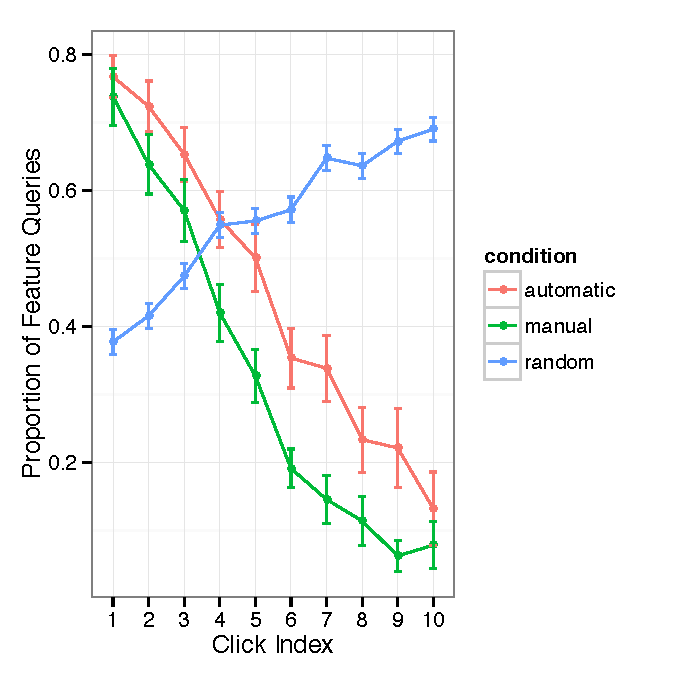
\includegraphics[width=0.4\textwidth]{figures/query_type_prop_by_click}
  \vspace{-.1cm}
  \caption{Proportion of feature vs. item queries by click for each update condition. People in both conditions are more likely to make feature queries rather than exemplar queries in the first three clicks of a round, but manual-update participants move more quickly to exemplar queries, and are overall more likely to make exemplar queries.}
  \label{fig:query-prop-click}
  \vspace{-.1cm}
\end{figure} 

\vspace{-.2cm}
\section{General Discussion}

Using a 20 questions style iterated binary search task with an unfamiliar but structured hypothesis space, this study investigated question asking strategies in children 5-10 years of age. Importantly, we manipulated the support children were given while updating the hypothesis space: after a feature query, participants in the automatic update condition were shown which bugs were eliminated at the press of a button, whereas manual update participants were required to select the bugs that were consistent with the feedback. 

Our qualitative analyses found that children use more constraint-seeking questions (i.e., feature queries) in the automatic-update condition. On the surface then, these children are using a more efficient strategy than the manual-update children. However, in terms of expected information gain, it turned out that children in the automatic-update condition were making less informative feature queries. We suggest that the greater mental effort required by the manual updating actually lead to more careful consideration of which feature query to use (indeed, RTs for feature queries were slower under manual updating), and ultimately a better choice.

\vspace{-.3cm}
\section{Acknowledgments}
\vspace{-.2cm}
This work was supported by the John Templeton Foundation ``Varieties of Understanding" grant to TMG and MR.
\vspace{-.2cm}
\bibliographystyle{apacite}

\setlength{\bibleftmargin}{.125in}
\setlength{\bibindent}{-\bibleftmargin}

\bibliography{sensemaking_refs}

\end{document}
